\documentclass[%
%10pt,
%varwidth=false,
%crop=true,
border={0mm 0mm 0mm 0mm}]{standalone}
\usepackage[T1]{fontenc}
\usepackage[utf8]{inputenc}
\usepackage[auto]{microtype}
%\usepackage{cmbright}
\usepackage{arev}
\usepackage{amsmath, amssymb, amsfonts, icomma}
\usepackage[version=4]{mhchem}
\usepackage{tikz}
\usetikzlibrary{positioning}
\usepackage{chemplants-tub}
\usepackage{xcolor}
%define stream tip, default is stealth
\setchpstreamtip{latex}
\setchpmainstreamthickness{thick}
%\setchpunitthickness{very thick}

\pgfdeclarelayer{bg}    % declare background layer
\pgfsetlayers{bg,main}  % set the order of the layers (main is the standard layer)

\definecolor{signalgruen}{RGB}{49,127,67}    % RAL 6032 Wasser
\definecolor{signalrot}{RGB}{155,36,35}      % RAL 3001 Dampf
\definecolor{signalgrau}{RGB}{150,153,146}   % RAL 7004 Luft
\definecolor{signalgelb}{RGB}{229,190,001}   % RAL 1003 brennbare und nicht brennbare Gase
\definecolor{signalorange}{RGB}{208,93,40}   % RAL 2010 Säuren
\definecolor{signalviolett}{RGB}{132,76,130} % RAL 4008 Laugen
\definecolor{signalbraun}{RGB}{121,77,62}    % RAL 8002 brennbare und nicht brennbare Flüssigkeiten
\definecolor{signalblau}{RGB}{30,45,110}     % RAL 5005 Sauerstoff

% TABLEAU-10
\definecolor{Tab10-A}{RGB}{78, 121, 167}
\definecolor{Tab10-B}{RGB}{242, 142, 43}
\definecolor{Tab10-C}{RGB}{225, 87, 89}
\definecolor{Tab10-D}{RGB}{118, 183, 178}
\definecolor{Tab10-E}{RGB}{89, 161, 79}
\definecolor{Tab10-F}{RGB}{237, 201, 72}
\definecolor{Tab10-G}{RGB}{176, 122, 161}
\definecolor{Tab10-H}{RGB}{255, 157, 167}
\definecolor{Tab10-I}{RGB}{156, 117, 95}
\definecolor{Tab10-J}{RGB}{186, 176, 172}

\begin{document}
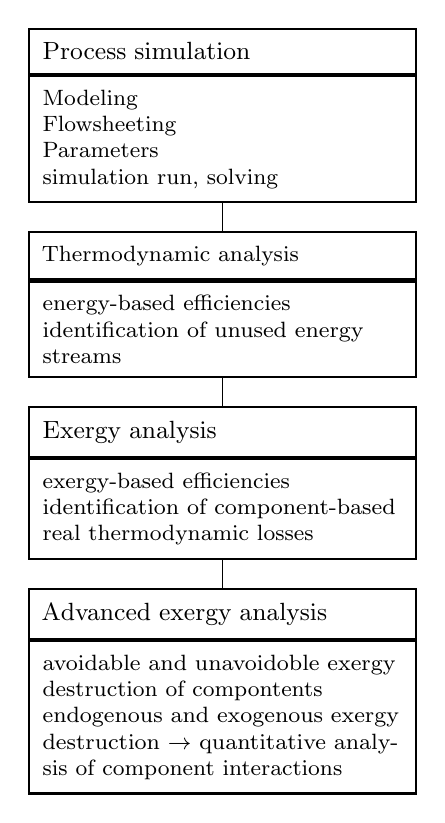
\begin{tikzpicture}[font=\footnotesize] 
%

%help grid and labels
%\draw[help lines] (-2,-3) grid (15,5);
%\foreach \pos in {-2,-1,0,1,2,3,4,5,6,7,8,9,10,11,12,13,14,15}
%\draw[shift={(\pos,-3)}] (0pt,2pt) -- (0pt,-2pt) node[below] {$\pos$};
%\foreach \pos in {-3,-2,-1,0,1,2,3,4,5}
%\draw[shift={(-2,\pos)}] (2pt,0pt) -- (-2pt,0pt) node[left] {$\pos$};

%%% nodes and boxes

%%% SIMULATION
\node [rectangle, draw=black, minimum width=140pt, text width= 130pt, thick, inner sep=5pt, align=left] (simulation) at (1,4) {\small Process simulation};
\node [rectangle, draw=black, minimum width=140pt, text width= 130pt, thick, inner sep=5pt, align=left, anchor=north] (simulation-sub) at (simulation.south) {Modeling\\
Flowsheeting\\
Parameters\\
simulation run, solving};

%%% TH. ANALYSIS
\node [rectangle, draw=black, minimum width=140pt, text width= 130pt, thick, inner sep=5pt, align=left, below = 10pt of simulation-sub] (th-analysis) {Thermodynamic analysis};
\node [rectangle, draw=black, minimum width=140pt, text width= 130pt, thick, inner sep=5pt, align=left, anchor=north] (th-analysis-sub) at (th-analysis.south) {energy-based efficiencies\\
identification of unused energy streams};

%%% EXERGY ANALYSIS
\node [rectangle, draw=black, minimum width=140pt, text width= 130pt, thick, inner sep=5pt, align=left, below = 10pt of th-analysis-sub] (exergy) {\small Exergy analysis};
\node [rectangle, draw=black, minimum width=140pt, text width= 130pt, thick, inner sep=5pt, align=left, anchor=north] (exergy-sub) at (exergy.south) {exergy-based efficiencies\\
identification of component-based real thermodynamic losses};

%%% ADV. EXERGY ANALYSIS
\node [rectangle, draw=black, minimum width=140pt, text width= 130pt, thick, inner sep=5pt, align=left, below = 10pt of exergy-sub] (adv-exergy) {\small Advanced exergy analysis};
\node [rectangle, draw=black, minimum width=140pt, text width= 130pt, thick, inner sep=5pt, align=left, anchor=north] (adv-exergy-sub) at (adv-exergy.south) {avoidable and unavoidoble exergy destruction of compontents\\
endogenous and exogenous exergy destruction $\rightarrow$ quantitative analysis of component interactions};



%%% connections, arrows

\draw [solid] (simulation-sub.south) -- (th-analysis.north);
\draw [solid] (th-analysis-sub.south) -- (exergy.north);
\draw [solid] (exergy-sub.south) -- (adv-exergy.north);

\end{tikzpicture}

\end{document}
